\section{Experiment Results}

\subsection{Evaluation Metrics}
We evaluate the classification performance of our proposed deep learning approaches
with the following metrics.
\begin{itemize}
    \item \textbf{Accuracy} is the percentage of correctly classified connections
        over the total number of connections in the dataset:
        \begin{align}
            A = \frac{\text{Correct Predictions}}{\text{Number of Records}}
        \end{align} 
        Accuracy is not suitable for evaluating biased dataset where the number
        of records of some class is extremely larger than the number of
        records of another class.
        In NSL-KDD dataset, the number of available U2R records (67)
        is in two degrees of magnitude less than the other classes of traffic (9711, 7458, 2887, 2121 respectively).
        Therefore we also consider the following metrics.
    \item \textbf{Precision} is the percentage of the correctly classified positives over
        the total number of positives predicted by the classifier:
                \begin{align}
                    P = \frac{\text{True Positives}}{\text{True Positives} + \text{False Positives}}
                \end{align}
    \item \textbf{Recall} is the percentage of the correctly classified positives over
        the total number of relevant elements:
                \begin{align}
                    R = \frac{\text{True Positives}}{\text{True Positives} + \text{False Negatives}}
                \end{align}
    \item \textbf{F1-Score} represents a balance between precision and recall and is calculated
        as their harmonic mean:
                \begin{align}
                    F = \frac{2PR}{P + R}
                \end{align}
\end{itemize}
In the 5-class classification, we calculate the precision, recall and F1-Score for each traffic class.
Additionally, we report the weighted average of these metrics as a single value for comparing various approaches.
The weight for each class is determined by its proportion in the test dataset.
The weight vector for class [Normal, Probe, DoS, U2R, R2L] is [0.431, 0.107, 0.339, 0.018, 0.105].
Besides, we also provide the confusion matrix of the classification results when applying
different approaches on the test dataset.
In our confusion matrix table, the row represents the instance in an actual class,
while the column represents the instance in a predicted class.
It is called confusion matrix because it is useful for visualizing how a classifier
is confusing one class with other class(es).


\subsection{Performance of Deep Learning Approaches}
First we report the classification accuracy of each considered approach in Figure~\ref{Fig:CompAccuracy}.
Surprisingly, the most ``accurate" approach is the simple forty-neuron perceptron (80.90\%).
Sparse autoencoder based self-taught leaner achieved second best accuracy of 79.15\%.
This number coincide with the previously reported results in~\cite{STL-NIDS} (79.10\%).
RBM and denoising autoencoder have similar accuracy results (77.58\% and 76.93\%).

\begin{figure}[h]
    \centering
    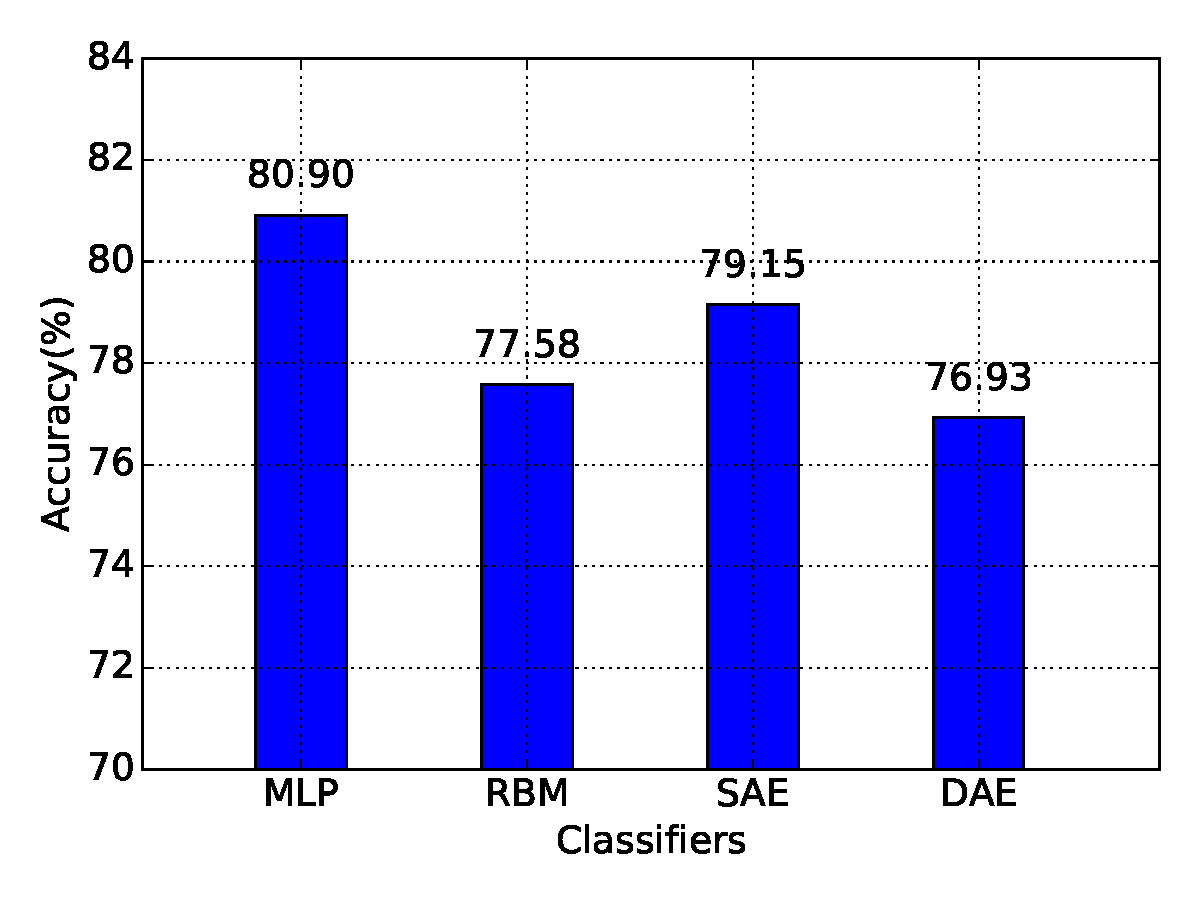
\includegraphics[width=0.48\textwidth]{figures/comp_accuracy.pdf}
    \caption{Classification Accuracy of Proposed Approaches}
    \label{Fig:CompAccuracy}
\end{figure}

Table~\ref{Tab:ConfusionMatrixMLP} --~\ref{Tab:ConfusionMatrixDAE} summarize the confusion matrix
of each approach and their weighted average metrics.
Apart from best accuracy, MLP also achieved the best F1-Score (79.64\%)
among all of the considered approaches.
However, we can see that for U2R attacks, MLP still has very poor results of
both precision (13.19\%) and recall (9.60\%).
The second highest F1-Score is achieved by sparse autoencoder combined with softmax regression (78.05\%).
This value is actually a little bit higher than the result (75.76\%) reported in~\cite{STL-NIDS}.
We believe this is partly due to the reason that we did not introduce regularization
for both sparse autoencoder and softmax regression classifier,
and partly due to the dropout technique we used in training the softmax regression classifier.
RBM and DAE again achieved very similar classification performance,
with F1-Score of 75.63\% and 75.65\% respectively.
Considering both the high accuracy and best F1-Score, we conclude that in the competition of
5-class classification, MLP is the winner.

Confusion matrices here tell us something interesting about the 
MLP correctly recognized the most number of normal traffics (9343 out of 9711).
For the attacking traffics, the winner classifier MLP correctly predicted the most
number of DoS attacks (6155 out of 7636).
RBM correctly identified the most number of Probe attacks (2015 out of 2425).
Both MLP and DAE correctly discovered the most number of U2R attacks (38 out of 396).
Sparse autoencoder identified the most number of R2L attacks correctly (895 out of 2376).

\begin{table}[t]
    \caption{Confusion Matrix of MLP on Test Dataset}
    \centering
    \begin{tabular}{cc|rrrrr}
        \hline
        &  & \multicolumn{5}{c}{Prediction} \\
                        &        & Normal & Probe & DoS & U2R & R2L\\
        \hline
        \hline
        \multirow{5}{*}{Actual} & Normal & {\color{red}9343} &  229 &   64 &  26 &  49 \\
                                &  Probe &  201 & 1925 &  227 &   9 &  63 \\
                                &  DoS   & 1332 &   68 & {\color{red}6155} &  47 &  34 \\
                                &  U2R   &  347 &    4 &    0 &  {\color{red}38} &   7 \\
                                &  R2L   & 1393 &   37 &    1 & 168 & 777 \\
        \hline
        \multicolumn{2}{c|}{Precision(\%)}   & 74.06 & 85.06 & 95.47 & 13.19 & 83.55\\
        \multicolumn{2}{c|}{Wtd. Avg.(\%)}   & \multicolumn{5}{r}{\color{red}82.43}\\
        \hline
        \multicolumn{2}{c|}{Recall(\%)}      & 96.21 & 79.38 & 80.61 &  9.6  & 32.7\\
        \multicolumn{2}{c|}{Wtd. Avg.(\%)}   & \multicolumn{5}{r}{\color{red}80.90}\\
        \hline
        \multicolumn{2}{c|}{F1-Score(\%)}    & 83.69 & 82.12 & 87.41 & 11.11 & 47.01\\
        \multicolumn{2}{c|}{Wtd. Avg.(\%)}   & \multicolumn{5}{r}{\color{red}79.64}\\
        \hline
    \end{tabular}
    \label{Tab:ConfusionMatrixMLP}
\end{table}


\begin{table}[t]
    \caption{Confusion Matrix of RBM on Test Dataset}
    \centering
    \begin{tabular}{cc|rrrrr}
        \hline
        &  & \multicolumn{5}{c}{Prediction} \\
                        &        & Normal & Probe & DoS & U2R & R2L\\
        \hline
        \hline
        \multirow{5}{*}{Actual} & Normal & 8903 &  318 &  428 &  11 &   51 \\
                                & Probe  &  232 & {\color{red}2015} &  159 &   2 &   17 \\
                                & DoS    & 1879 &  143 & 5613 &   0 &    1 \\
                                & U2R    &  356 &    3 &    1 &  27 &    9 \\
                                & R2L    & 1550 &    8 &    1 &   8 &  809 \\
        \hline
        \multicolumn{2}{c|}{Precision(\%)}   & 68.91& 81.02& 90.50& 56.25& 91.21\\
        \multicolumn{2}{c|}{Wtd. Avg.(\%)}   & \multicolumn{5}{r}{79.65}\\
        \hline
        \multicolumn{2}{c|}{Recall(\%)}      & 91.68& 83.09& 73.51&  6.82& 34.05\\
        \multicolumn{2}{c|}{Wtd. Avg.(\%)}   & \multicolumn{5}{r}{77.04}\\
        \hline
        \multicolumn{2}{c|}{F1-Score(\%)}    & 78.68& 82.04& 81.12& 12.16& 49.59\\
        \multicolumn{2}{c|}{Wtd. Avg.(\%)}   & \multicolumn{5}{r}{75.63}\\
        \hline
    \end{tabular}
    \label{Tab:ConfusionMatrixRBM}
\end{table}

\begin{table}[t]
    \caption{Confusion Matrix of SAE on Test Dataset}
    \centering
    \begin{tabular}{cc|rrrrr}
        \hline
        &  & \multicolumn{5}{c}{Prediction} \\
                        &        & Normal & Probe & DoS & U2R  & R2L\\
        \hline
        \hline
        \multirow{5}{*}{Actual}  & Normal & 8864 &  696 &   92 &   11 &   48 \\
                                 & Probe  &  179 & 2001 &  164 &    2 &   79 \\
                                 & DoS    & 1542 &   39 & 6054 &    0 &    1 \\
                                 & U2R    &  357 &    1 &    1 &   30 &    7 \\
                                 & R2L    & 1444 &    6 &    5 &   26 &  {\color{red}895} \\
        \hline
        \multicolumn{2}{c|}{Precision(\%)}    & 71.56& 72.95& 95.85& 43.48& 86.89\\
        \multicolumn{2}{c|}{Wtd. Avg.(\%)}    & \multicolumn{5}{r}{81.06}\\
        \hline
        \multicolumn{2}{c|}{Recall(\%)}       & 91.28& 82.52& 79.28&  7.58& 37.67\\
        \multicolumn{2}{c|}{Wtd. Avg.(\%)}    & \multicolumn{5}{r}{79.15}\\
        \hline
        \multicolumn{2}{c|}{F1-Score(\%)}     & 80.23& 77.44& 86.78& 12.90& 52.55\\
        \multicolumn{2}{c|}{Wtd. Avg.(\%)}    & \multicolumn{5}{r}{78.05}\\
        \hline
    \end{tabular}
    \label{Tab:ConfusionMatrixSAE}
\end{table}


\begin{table}[t]
    \caption{Confusion Matrix of DAE on Test Dataset}
    \centering
    \begin{tabular}{cc|rrrrr}
        \hline
        &  & \multicolumn{5}{c}{Prediction} \\
                        &        & Normal & Probe & DoS & U2R & R2L\\
        \hline
        \hline
        \multirow{5}{*}{Actual} & Normal & 9249 &  319 &   85 &  10 &  48 \\
                                & Probe  & 576  & 1504 &  226 &   2 & 117 \\
                                & DoS    & 1842 &  128 & 5665 &   0 &   1 \\
                                & U2R    & 353  &    1 &    0 &  {\color{red}38} &   4 \\
                                & R2L    & 1469 &    3 &    1 &  17 & 886 \\
        \hline
        \multicolumn{2}{c|}{Precision(\%)} & 68.57& 76.93& 94.78& 56.72& 83.90\\
        \multicolumn{2}{c|}{Wtd. Avg.(\%)} & \multicolumn{5}{r}{79.75}\\
        \hline
        \multicolumn{2}{c|}{Recall(\%)}    & 95.24& 62.02& 74.19&  9.60& 37.29\\
        \multicolumn{2}{c|}{Wtd. Avg.(\%)} & \multicolumn{5}{r}{76.93}\\
        \hline
        \multicolumn{2}{c|}{F1-Score(\%)}  & 79.73& 68.68& 83.23& 16.41& 51.63\\
        \multicolumn{2}{c|}{Wtd. Avg.(\%)} & \multicolumn{5}{r}{75.65}\\
        \hline
    \end{tabular}
    \label{Tab:ConfusionMatrixDAE}
\end{table}

